\chapter{Synchroniczny przerzutnik RS}

\section{Budowa układu}

\begin{itemize}
    \item Należało zbudować przerzutnik synchroniczny RS korzystając ze schematu (\ref{przerzutnik_RS:schemat}) korzystającego z 4 bramek NAND (\ref{tabela_prawdy:NAND}) z czego 2 były dwuwejściowe (TTL 7400 (\ref{link:7400})) oraz 2 trójwejściowe (TTL 7410 (\ref{link:7410}))
        \begin{figure}[H]
            \centering
            \begin{subfigure}[H]{0.45\textwidth}
                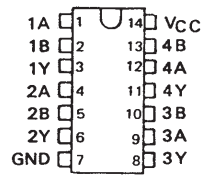
\includegraphics[width=\textwidth]{img/schemes/7400_pins.png}
                \caption{Piny TTL 7400}
            \end{subfigure}
            \begin{subfigure}[H]{0.45\textwidth}
                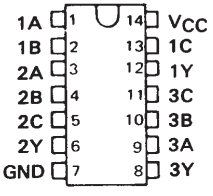
\includegraphics[width=\textwidth]{img/schemes/7410_pins.png}
                \caption{Piny TTL 7410}
            \end{subfigure}
        \end{figure}
    \item Do wejść \textbf{c} oraz \textbf{d} (patrz: \ref{przerzutnik_RS:schemat}) podpięto logiczne 0 lub 1 korzystając z pinów 5V oraz 0V na płytce oraz rezystorów 1k$\Omega$ oraz 400$\Omega$:
        \begin{center}
            Łącząc opornik 1k$\Omega$ z wejściem 5V uzyskujemy logiczne 1. \\
            Łącząc opornik 400$\Omega$ z wejściem 0V uzyskujemy logiczne 0.
        \end{center}
    \item Górny impulsator służy do przesyłania sygnałów do wejść \textbf{a}, \textbf{b} (patrz: \ref{przerzutnik_RS:schemat})
    \item Dolny impulsator służy jako zegar.
    \item Wyjście przerzutnika \textbf{Q} oraz $\overline{\textbf{Q}}$ (piny 6, 8) zostały wyprowadzone do diod elektroluminescencyjnych znajdujących się na prawej stronie płytki.
        \begin{figure}[H]
            \centering
            \begin{subfigure}[H]{0.45\textwidth}
                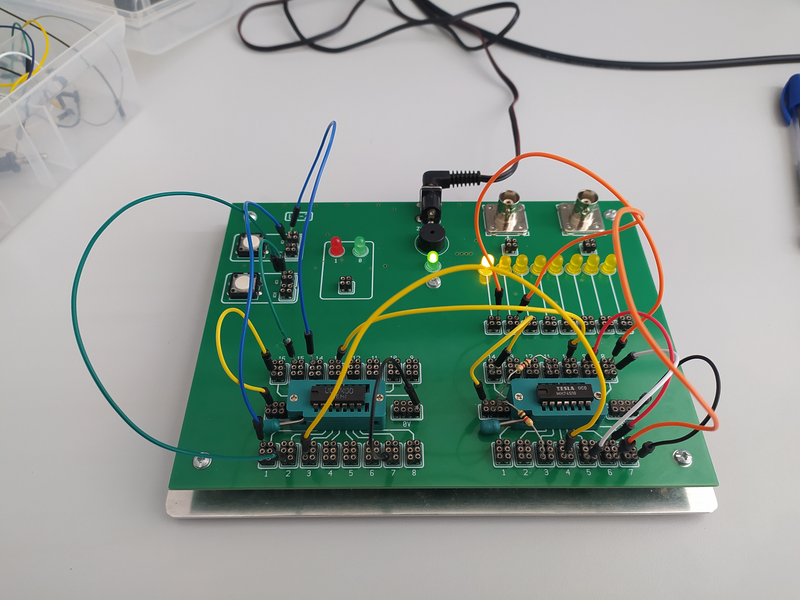
\includegraphics[width=\textwidth]{img/synch_RS/1653500525466_scaled.png}
            \end{subfigure}
            \begin{subfigure}[H]{0.45\textwidth}
                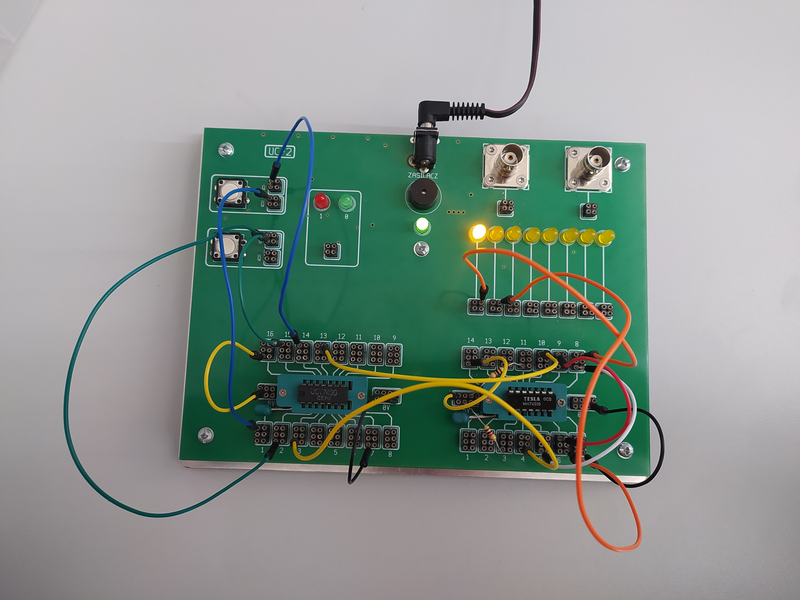
\includegraphics[width=\textwidth]{img/synch_RS/1653500525452_scaled.png}
            \end{subfigure}
            \caption{Zbudowany przerzutnik synchroniczny RS}
        \end{figure}
    
        \begin{figure}[H]
            \centering
            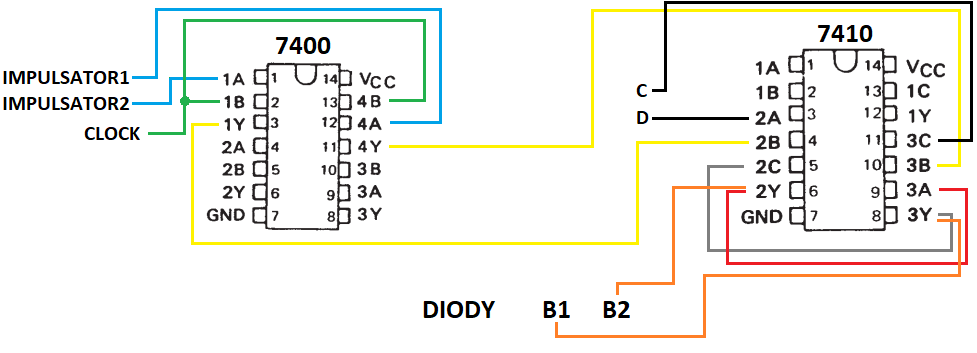
\includegraphics[width=\textwidth]{img/schemes_w_pins/RS_w_pins.png}
            \caption{Schemat z połączonymi pinami}
            \label{RS:schemat_z_pinami}
        \end{figure}
\end{itemize}

\section{Test}

\begin{itemize}
    \item Przetestowano zbudowany przerzutnik dla różnych wartości \textbf{c}, \textbf{d}.
    \item \textbf{c = 1}, \textbf{d = 1}:
        %1653500525398_scaled
        \begin{figure}[H]
            \centering
            \begin{subfigure}[H]{0.4\textwidth}
                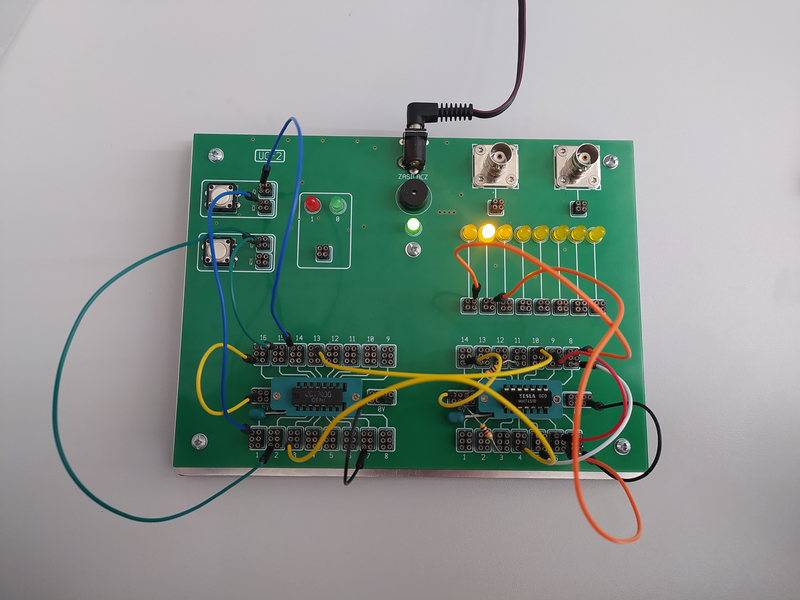
\includegraphics[width=\textwidth]{img/synch_RS/1653500525439_scaled.png}
            \end{subfigure}
            \begin{subfigure}[H]{0.4\textwidth}
                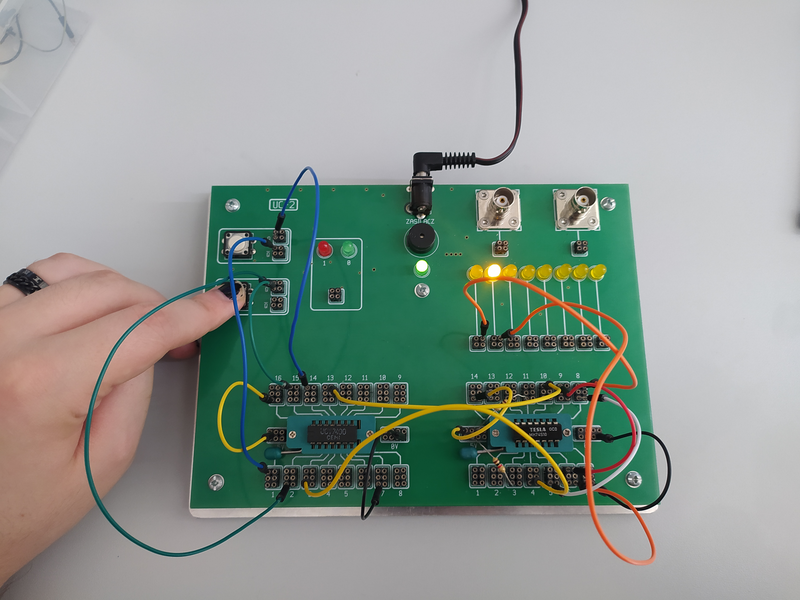
\includegraphics[width=\textwidth]{img/synch_RS/1653500525417_scaled.png}
            \end{subfigure}
            \begin{subfigure}[H]{0.4\textwidth}
                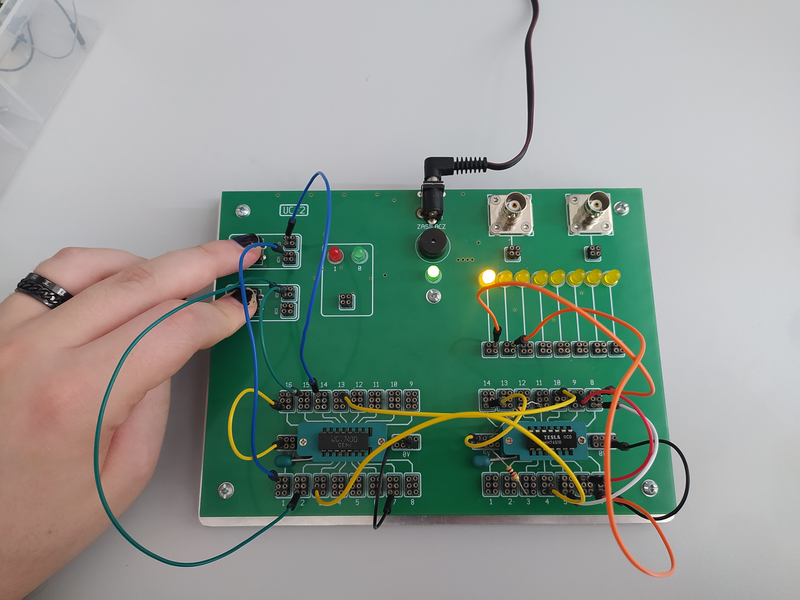
\includegraphics[width=\textwidth]{img/synch_RS/1653500525408_scaled.png}
            \end{subfigure}
            \begin{subfigure}[H]{0.4\textwidth}
                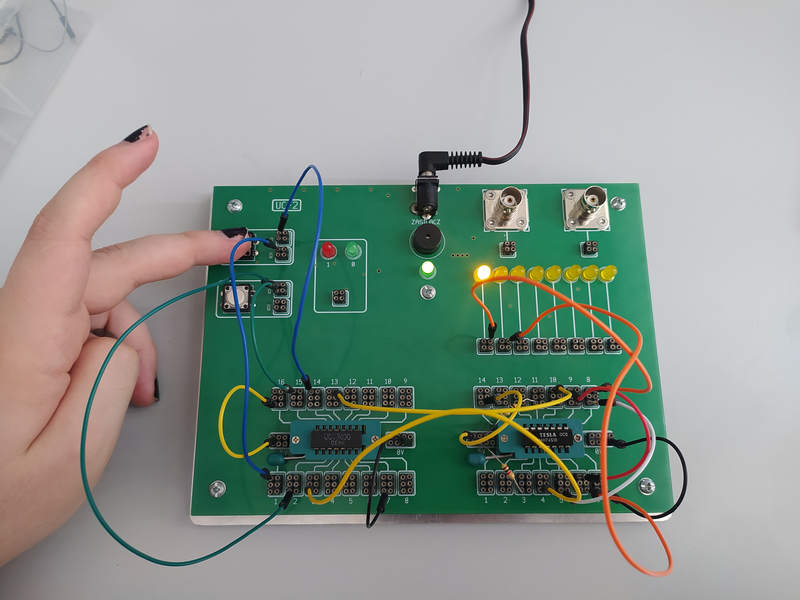
\includegraphics[width=\textwidth]{img/synch_RS/1653500525398_scaled.png}
            \end{subfigure}
            \caption{Testowanie przerzutnika synchronicznego RS}
        \end{figure}

        Układ dla tych wartości c,d \textbf{poprawnie}.

\pagebreak

    \item \textbf{c = 0}, \textbf{d = 1}:
        \begin{figure}[H]
            \centering
            \begin{subfigure}[H]{0.4\textwidth}
                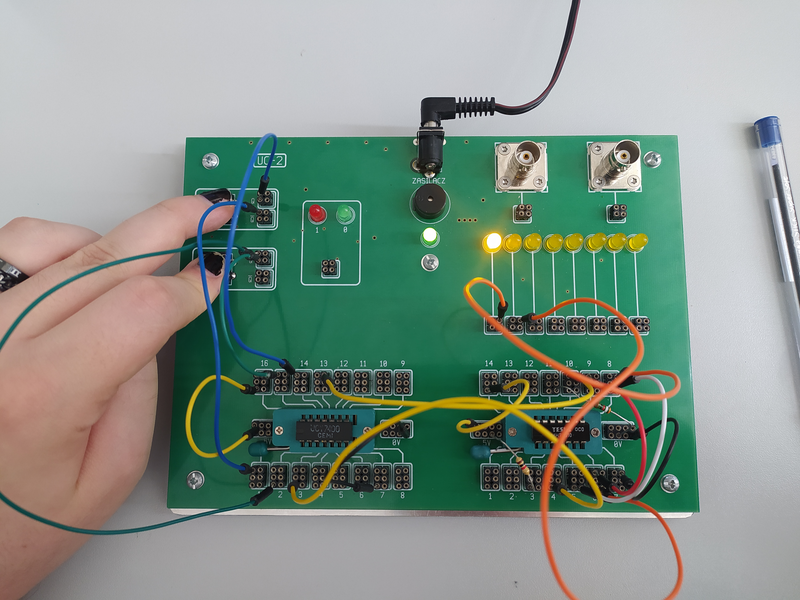
\includegraphics[width=\textwidth]{img/synch_RS/1653500525344_scaled.png}
            \end{subfigure}
            \begin{subfigure}[H]{0.4\textwidth}
                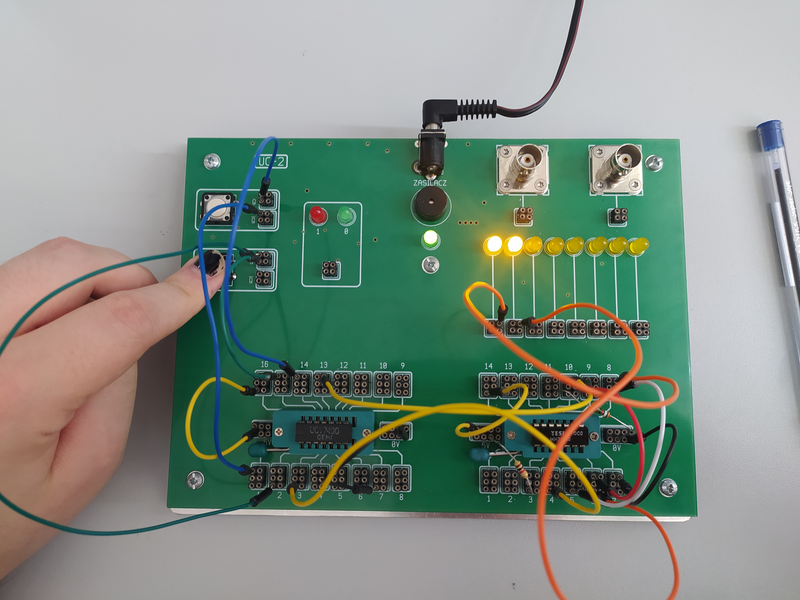
\includegraphics[width=\textwidth]{img/synch_RS/1653500525359_scaled.png}
            \end{subfigure}
        \end{figure}

        Układ dla tych wartości c,d \textbf{poprawnie}.

    \item \textbf{c = 1}, \textbf{d = 0}:
        \begin{figure}[H]
            \centering
            \begin{subfigure}[H]{0.4\textwidth}
                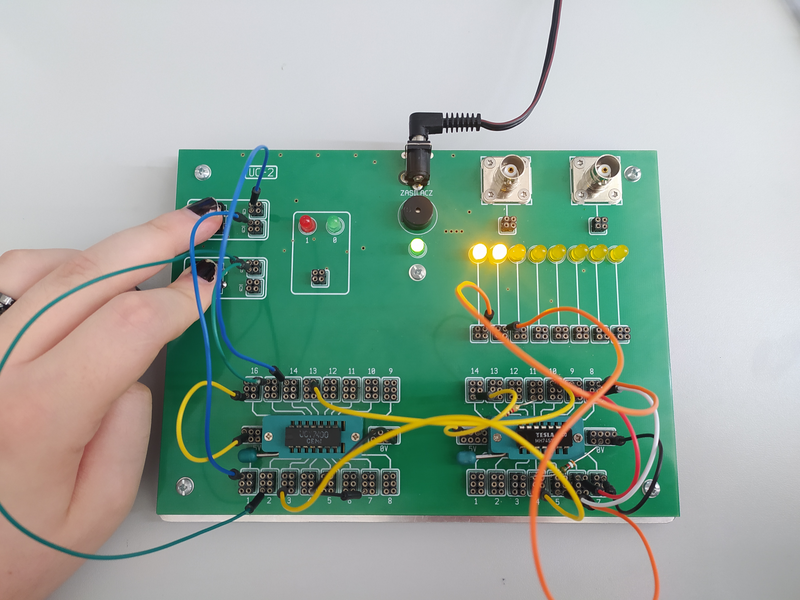
\includegraphics[width=\textwidth]{img/synch_RS/1653500525372_scaled.png}
            \end{subfigure}
            \begin{subfigure}[H]{0.4\textwidth}
                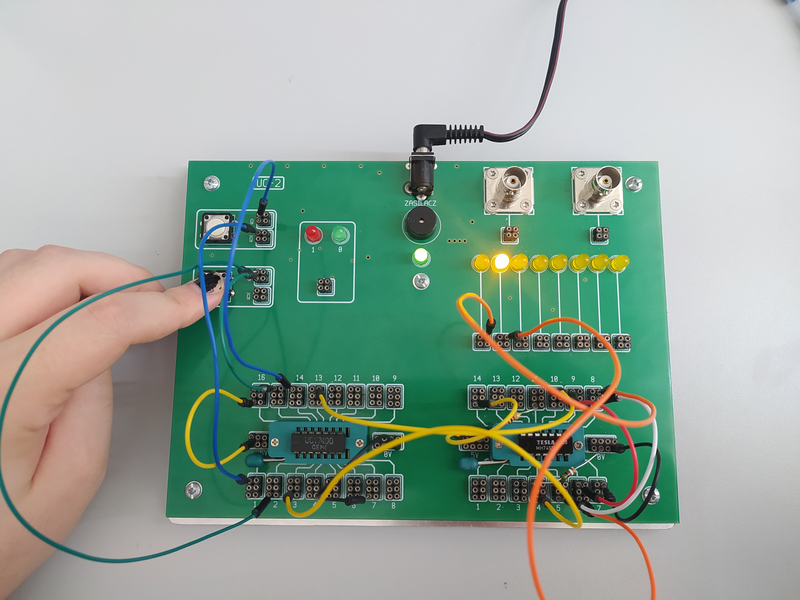
\includegraphics[width=\textwidth]{img/synch_RS/1653500525388_scaled.png}
            \end{subfigure}
        \end{figure}

        Układ dla tych wartości c,d \textbf{poprawnie}.
\end{itemize}

\section{Podpięcie generatora funkcyjnego}

\begin{itemize}
    \item Zastąpiono zegar wywoływany sygnałem impulsatora sygnałem prostokątnym z generatora funkcyjnego. 
    \item Generatorem funkcyjnym generowano sygnał prostokątny o zadanych wartościach:
        \begin{figure}[H]
            \centering
            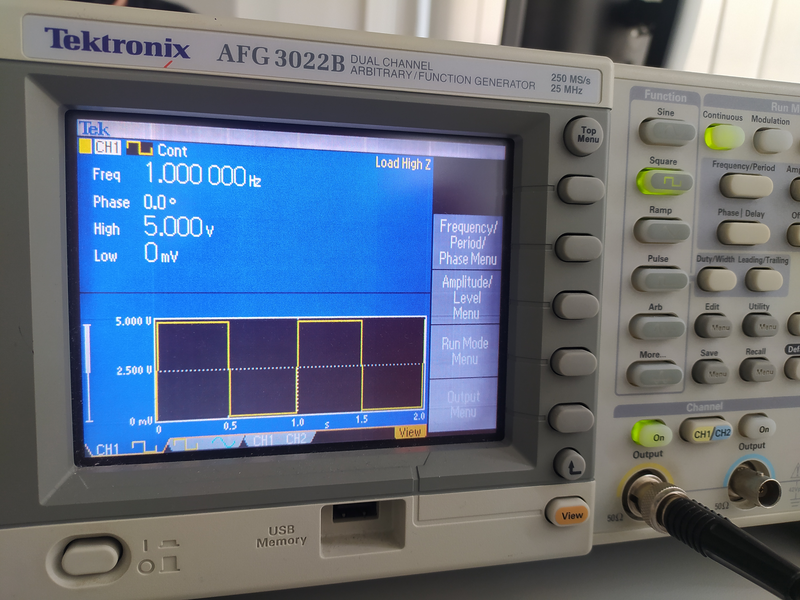
\includegraphics[width=0.4\textwidth]{img/synch_RS/1653500525328_scaled.png}
            \caption{Sygnał prostokątny, T=\textbf{1s}, $U_{low}$ = \textbf{0V}, $U_{high}$ = \textbf{5V}}
            \label{fig:my_label}
        \end{figure}
    \item Wyjście z generatora funkcyjnego poprowadzono do próbnika logicznego aby zaobserwować zmieniające się co sekundę logiczne wartości.
        \begin{figure}[H]
            \centering
            \begin{subfigure}[H]{0.4\textwidth}
                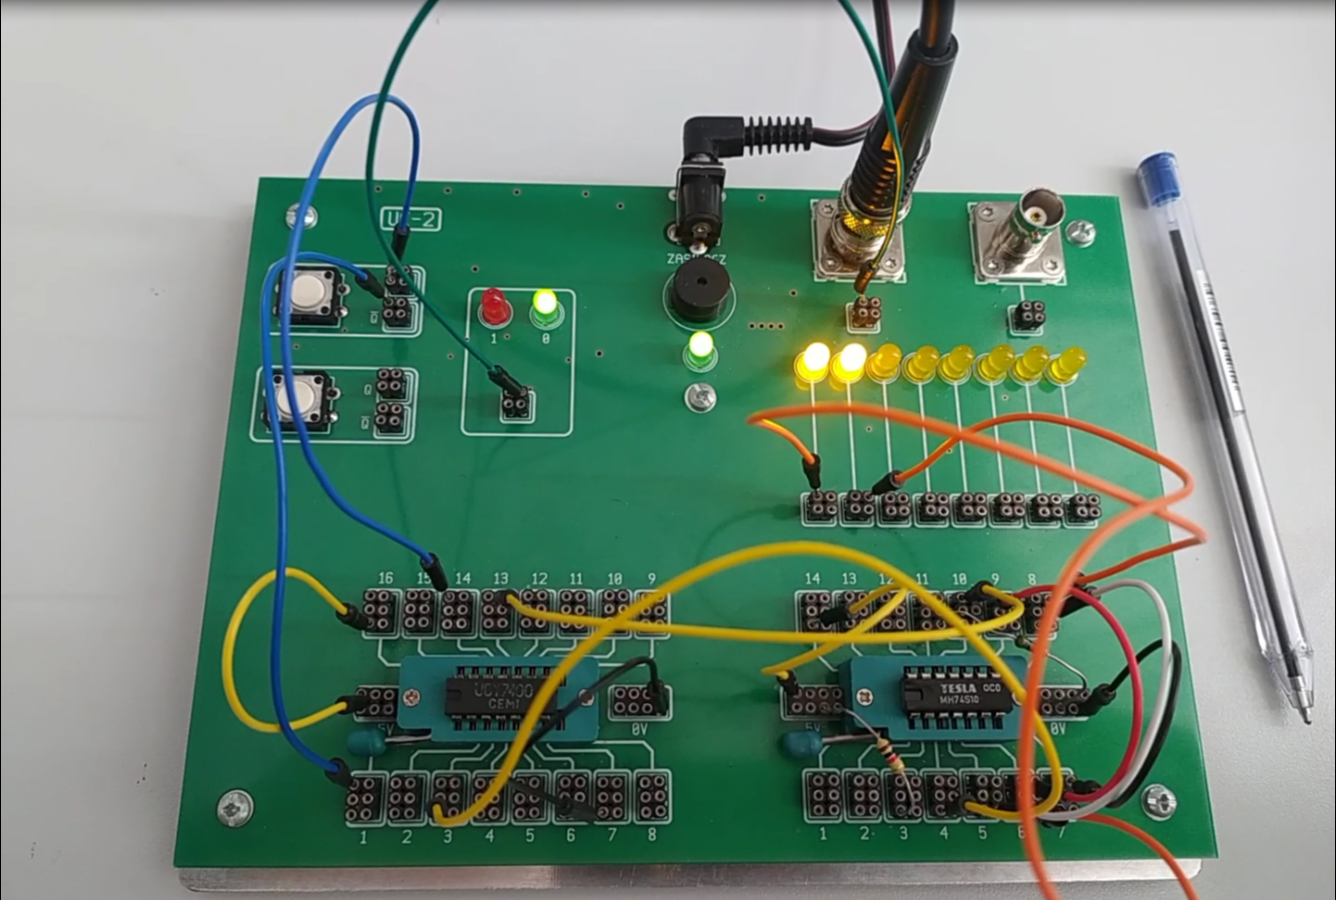
\includegraphics[width=\textwidth]{img/synch_RS/generator_0.png}
                \caption*{Logiczne 0}
            \end{subfigure}
            \begin{subfigure}[H]{0.4\textwidth}
                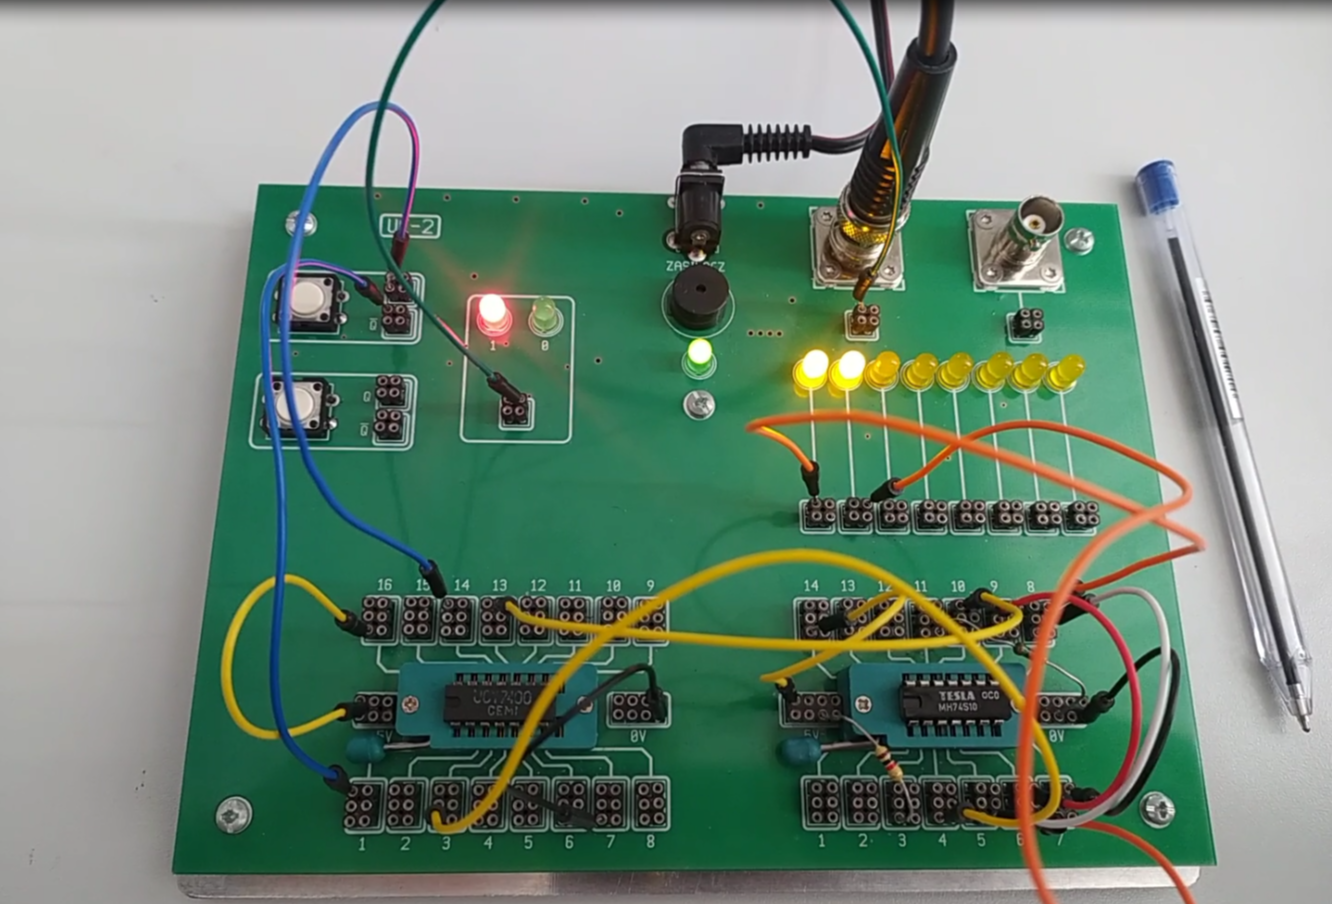
\includegraphics[width=\textwidth]{img/synch_RS/generator_1.png}
                \caption*{Logiczne 1}
            \end{subfigure}
        \end{figure}
    \item Następnie podpięto sygnał z generatora do wejścia zegara w przerzutniku synchronicznym RS.
        \begin{figure}[H]
            \centering
            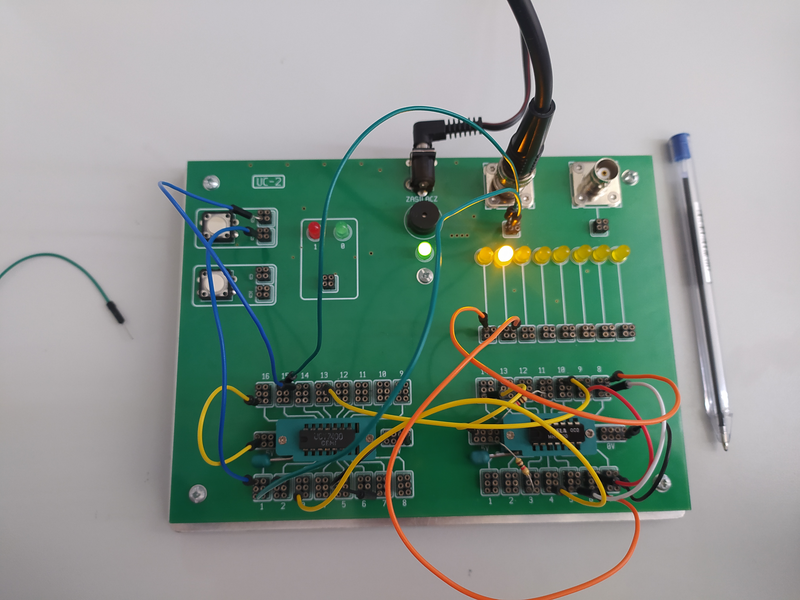
\includegraphics[width=0.7\textwidth]{img/synch_RS/1653500525164_scaled.png}
            \caption{Synchroniczny przerzutnik RS z zegarem z generatora funkcyjnego}
            \label{fig:my_label}
        \end{figure}
    \item Układ z podpiętym zegarem z generatora funkcyjnego działał \textbf{poprawnie}.
\end{itemize}